\documentclass[conference]{IEEEtran}
\IEEEoverridecommandlockouts
% The preceding line is only needed to identify funding in the first footnote. If that is unneeded, please comment it out.
\usepackage{cite}
\usepackage{amsmath,amssymb,amsfonts}
\usepackage[T1]{fontenc}
\usepackage{algorithmic}
\usepackage{amsmath,amssymb,amsfonts}
\usepackage{graphicx}
\usepackage{textcomp}
\usepackage{xcolor}
\usepackage{listings}
\usepackage{hyperref}
\usepackage{subcaption}
\usepackage{caption}
\usepackage{multirow}
\usepackage{float}
\usepackage[normalem]{ulem}

\def\BibTeX{{\rm B\kern-.05em{\sc i\kern-.025em b}\kern-.08em
    T\kern-.1667em\lower.7ex\hbox{E}\kern-.125emX}}
\begin{document}

\title{MACHINE LEARNING APPROACH FOR THE PREDICTION OF THE STATUS OF TANZANIAN WELLS [COMP4030 CW2 - Data Science and Machine Learning]
}

\author{\IEEEauthorblockN{*Thomas Cotter}
\IEEEauthorblockA{\textit{Computer Science} \\
\textit{University of Nottingham}\\
Nottingham, England\\
psytc8@nottingham.ac.uk}
\and
\IEEEauthorblockN{*Loo Yang Shen Jason}
\IEEEauthorblockA{\textit{Computer Science} \\
\textit{University of Nottingham}\\
Nottingham, England \\
hfyyl5@nottingham.ac.uk}
}

\maketitle

\begin{abstract}
  This paper details our approaches and results for the COMP4030 CW2. The goal was to predict the status ('Functional', 'Functional - Needs Repair' \& 'Non-Functional') of water wells in Tanzania. This is important as not only does knowing the status of the well help keep the total percentage of functioning wells higher, but it also allows for more effective spending on repairs. The most important features included 'age', 'season\_when\_recorded', 'height\_above\_sealevel' \& 'extraction\_type'. The best performing models were XGBoost and VotingClassifier.
\end{abstract}

\begin{IEEEkeywords}
  Machine Learning, Data Science, Classification, Water Pumps
\end{IEEEkeywords}

\section{Introduction}

\subsection{Research Questions}

\textbf{What factors are most important for determining the status of a well, and how accurately can we classify wells based on these features?}. 

We choose this question because we are interested in the factors that determine the status of a well, and using ML to try to classify these wells. Follow-up questions to this question could include:
    \begin{itemize}
        \item How does the accuracy of the classification model vary with different feature sets and classification algorithms?
        \item Could we use our results to ensure that wells are built and repaired so that fewer wells are non-functional?
    \end{itemize}

\subsection{Dataset}

The chosen dataset is from the Tanzanian Ministry of Water and contains information on the status of wells in Tanzania. This dataset has 59400 rows, with 40 different features. These 40 features could be broken down into three subgroups: a) Geographic Location of the Wells. b) Management of the wells. and c) Water Condition of the wells.

Fig. \ref{fig:status_groups} shows the distribution of the target variable, which is the status of the well. We can see from this that we might need to oversample the 'functional needs repair' class, due to class imbalance.

\begin{figure}[h]
    \centering
    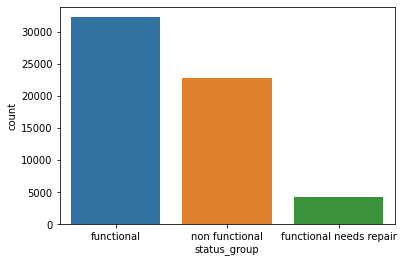
\includegraphics[scale=0.5]{figures/status_groups.png}
    \caption{Distribution of the target variable}
    \label{fig:status_groups}
\end{figure}

\subsection{Management Structure}

A requirement of this project was to work separately within our pairs and try different techniques to solve the problem. To not lose important insights, we communicated our results throughout the project. We followed a 'Christmas Tree'-like approach for each stage: 'Data Analysis', 'Data Pre-processing' \& 'Data Classification'. Each section was performed individually, before combining our results and moving out the next section. This process was performed cyclically, re-visiting steps when required. See Fig. \ref{fig:management_structure}

\begin{figure}[h]
    \centering
    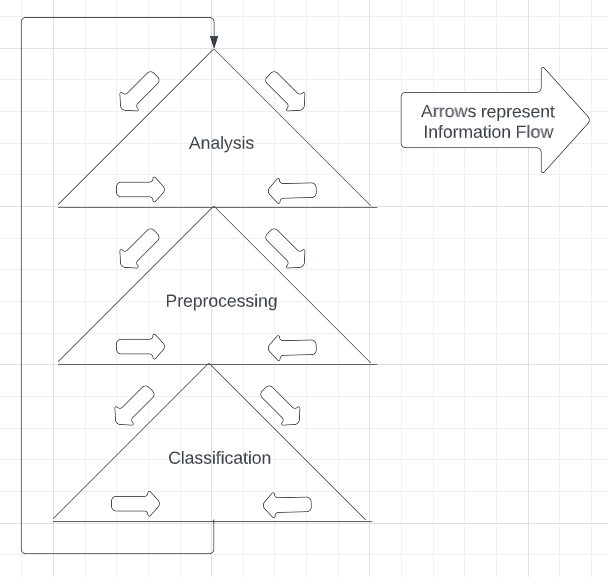
\includegraphics[scale=0.3]{figures/ct_approach.png}
    \caption{Management Structure}
    \label{fig:management_structure}
\end{figure}

This results in two main benefits. Firstly, it allows us to research a large number of approaches, which provides a higher chance of finding a powerful approach. Secondly, the combination of approaches that resulted may provide more optimal results. 

\section{Literature Review}

One study by Pathak et al. (2023) \cite{pathak2023pump} compared the performance of TabNet, a sequential attentive classification architecutre designed for tabular data, and tree-based approaches such as XBBoost. They found that TabNet outpeformed XGBoost, boasting an 83\% accuracy compared to XGBoosts 78\%. TabNet makes use of Transformers, a machine learning algorithm which uses self-attention to differentially weight the significance of each part of the input. A point of note is that TabNet does not require feature engineering to perform at these standards. We have not used TabNet in our report, as our primary goal was to showcase an end-to-end machine learning solution, and this includes feature enginering. However, it provides an interesting comparision.

Pham et al studied fully connected neural networks on the Pump it Up dataset \cite{Pham_2018}, settling on a model with 7 hidden layers and cross-entropy loss as the loss function. Their trained model achieved a 78.6\% accuracy rate on the test dataset. Although our project has prioritized tree-based methods for their speed, it would be interesting to compare our results with those of a neural network.

Jithin Paul also undertook a study on the Pump it Up dataset, experimenting with different models to test for the best results \cite{Paul_2023}. He proposed four methods, RandomForest, DeepLearning, LogisticRegression \& AdaBoost. The results showed that RandomForest, was the most accurate model, achieving a mean accuracy of 81.18\% on the test dataset. This finding demonstrates that tree-based models perform exceptionally well on this dataset, which motivated us to use more sophisticated tree-based methods in our own work.

\section{Methodology} \label{ref:method}

\subsection{Data Analysis}


When conducting data analysis, the python library Seaborn \cite{seaborn} was our primary data visualization tool. Seaborn offers more visually appealing graphs than MatPlotLib.

\subsubsection{Thomas}

Thomas visualized the correlation between 'construction\_year'and other features in the dataset. 'construction\_year' had a number of missing values, therefore these graphs could determine the possibility of using other features to impute the missing values.

\subsubsection{Jason}

Jason checked the number of missing and unique values across 38 features provided to identify features that would require imputation. In addition, this step allowed him to distinguish features which would have to be recategorised due to the large number of unique values present. He also generated countplots for each of the previously mentioned features based on water wells' status. These plots allowed him to visualise the distribution of the wells' status based on features. Thus, making it easier to identify features that could possibly influence the status of a water well.

\subsection{Data Preprocessing}

\subsubsection{Thomas}

Thomas performed imputation of the lat \& lon missing values by applying grouped mean imputation. The data was grouped by 'ward', 'lga' and then 'region'. This ensured that any missing values in either 'ward' or 'lga' did not result in missing lat / lon values. This provides more accurate results than 'regular' mean imputation, as the imputed values are localised. The Funder \& Installer columns contained 1000s of unique values. In Thomas' approach, he decided to group the column into categories: 'Charity', 'Government', 'Local Government', 'Private', 'Religious', 'Foreign', 'School' \& 'Unknown'. This was done to simplify the dataset, making it easier for the model to learn the distribution. Since, the columns had crossover between the values, this can be done in 1 step. Thomas also used the SMOTE-ENN algorithm from imblearn \cite{smote-enn}, to balanced the dataset, specificall the 'Functional - Needs Repair' class. Imbalanced datasets could potentially affect model performance, especially in tree-based models. Finally, 'gps-height' was normalised using a custom MinMaxScaler and a custom Z-Score Scaler. This was due to the prevelence of outliers in the 'gps-height' feature.

\subsubsection{Jason}

Due to the presence of missing data in the Latitude \& Longitude columns, Jason decided to apply mean imputation based on the Region column. By calculating the mean lat and lon value of each region, a rough estimation of the  location of wells with missing values could be known. 

During Data Analysis, he noticed the Permit and Public Meeting columns had missing values. Upon further inspection, these two columns only contain the values of either 'True' or 'False'. Data Imputation was not done here due to the lack of valuable data present in the data set. To preserve the distribution of these two columns, a unique values known as 'Unknown' was given to rows with missing data.

He performed data recategorisation on both funder and installer columns which contained 1000s of unique values. He performed data cleaning to fix spelling mistakes that were present in each column. This was followed categorizing each value with a count of less than 1000 as 'Other'. Each unique value above a count of 1000 became it's own category. Data recategorisation might improve the models' training perforamance.

He decided to reclassify the values in the region column according to their geographical zones based on data that was provided by the Tanzania Water and Sanitation Network \cite{tawasanet}. This reduced the number of unique values of the Region Column to 7 from 21. New insights could potentially be drawn upon based on the zone that the water wells is currently located in.

The data set provided had feature and target variables in the form of categorical form. he had converted these features into numerical form required by ML models. Each value was encoded in alphabetical order whereby a = 0, b = 1 etc. 

\subsection{Data Classification}

Initially, we focused on testing the performance of different algorithms without any feature selection. This allows us to focus on the best performing ones. See Table. \ref{tab:initial-clf-results}. We can see that XGBoostClassifier, CatBoostClassifier, BaggingClassifier \& HistGradientBoostingClassifier were the most effective for our problem. We decided to explore these models using feature selection \& hyper-parameter tuning. Our feature selection process employed a Chi-Squared test and feature importances obtained from a RandomForest and a XGBoost.

\begin{table}[h]
  \centering
  \caption{Initial Classification Results}
  \label{tab:initial-clf-results}
  \begin{tabular}{|c|c|c|c|}
    \hline
    \textbf{Algorithm} & \textbf{Accuracy} & \textbf{Precision} & \textbf{Recall} \\ \hline
    XGB	& \textbf{0.799} & \textbf{0.751} & 0.633 \\
    \hline
    CatBoost & 0.795 & 0.746 & 0.634 \\
    \hline
    Bagging & 0.793 & 0.704 & \textbf{0.659} \\
    \hline
    HistGradientBoosting & 0.791 & 0.743 & 0.624 \\
    \hline
    DT & 0.757 & 0.643 & 0.645 \\
    \hline
    KNN & 0.709 & 0.623 & 0.563 \\
    \hline
  \end{tabular}
\end{table}


\subsubsection{Thomas}

Thomas trained the 4 top models (XGBoost, CatBoost, Bagging \& HGBoost) on the SMOTE balanced dataset and compared the results to models trained on the imbalanced dataset. The results were also compared when optimizing for 'recall\_macro' or 'accuracy'. Recall is usually a better metric for imbalanced datasets, as accuracy can often misrepresent the truth. 'recall\_macro' takes an average of the recall for all 3 classes, which makes it a good metric to use.

Furthermore, he used Weights and Biases (WandB) \cite{wandb} to analyse the subset of features produced by the Chi-Squared Test and RandomForest. WandB served as an accesible MLOps platform for experiment tracking. Multiple classifiers were trained on different feature subsets (ranging from sizes 0.75N to N, where N is the size of the original feature set), and tracked this information in WandB. WandB allows us to quickly filter for the best performing 'runs', and the feature subset used. He also used WandB to further analyse the results of his cross-validation hyper-parameter tuning, in much a similar process to feature selection.

\subsubsection{Jason}

From the Random Forest feature importance and Chi-Squared Test, Jason shortlisted 16 features. Prior to model training, the dataset was subjected to a 80\%:20\% train test split. This was followed by normalising the testing and training set features with z-score normalisation.

For this study, he considered three different ML models  (Random Forrest, XGBoost \& CatBoost). Hyperparameter tuning was conducted via GridSearchCV \cite{gridsearch}. The most optimal parameters of each model were recorded before being passed for model training. 

To evaluate the performance of each model, K-fold cross validation (CV) with k=5, confusion matrix and receiver operating characteristic (ROC) curve were used. K-fold cross validations CV was used to evaluate the performance of the model on unseen data. Meanwhile, confusion matrix showcases the predictions which are labelled correctly and incorrectly by class. Although ROC Curves are usually meant for binary classification, it was extended to  be used for multiclass classification through pairwise comparison i.e., one class vs all other classes.   

\section{Results} \label{ref:results}

All results are rounded to 2 or 3 significant figures. The best performing model is highlighted in bold.

\subsection{Data Analysis}

\subsubsection{Thomas}

An example of the construction year visulisations can be see in Fig. \ref{fig:construction_year}. From this, we can see that there is a slight variation in Waterpoint Type usage across decades, but nothing of significance. The same is true across the other visualisations produced (see the accompanying ipynb for more details). For this reason, the missing values in the Construction year were kept as 'Unknown'. The distribution of the status group values in 'Unknown' or 'Not Unknown' construction year values can be seen in Fig \ref{fig:construction_year}.

\begin{figure*}[t!]
    \centering
    \begin{subfigure}[t]{0.5\textwidth}
      \centering
      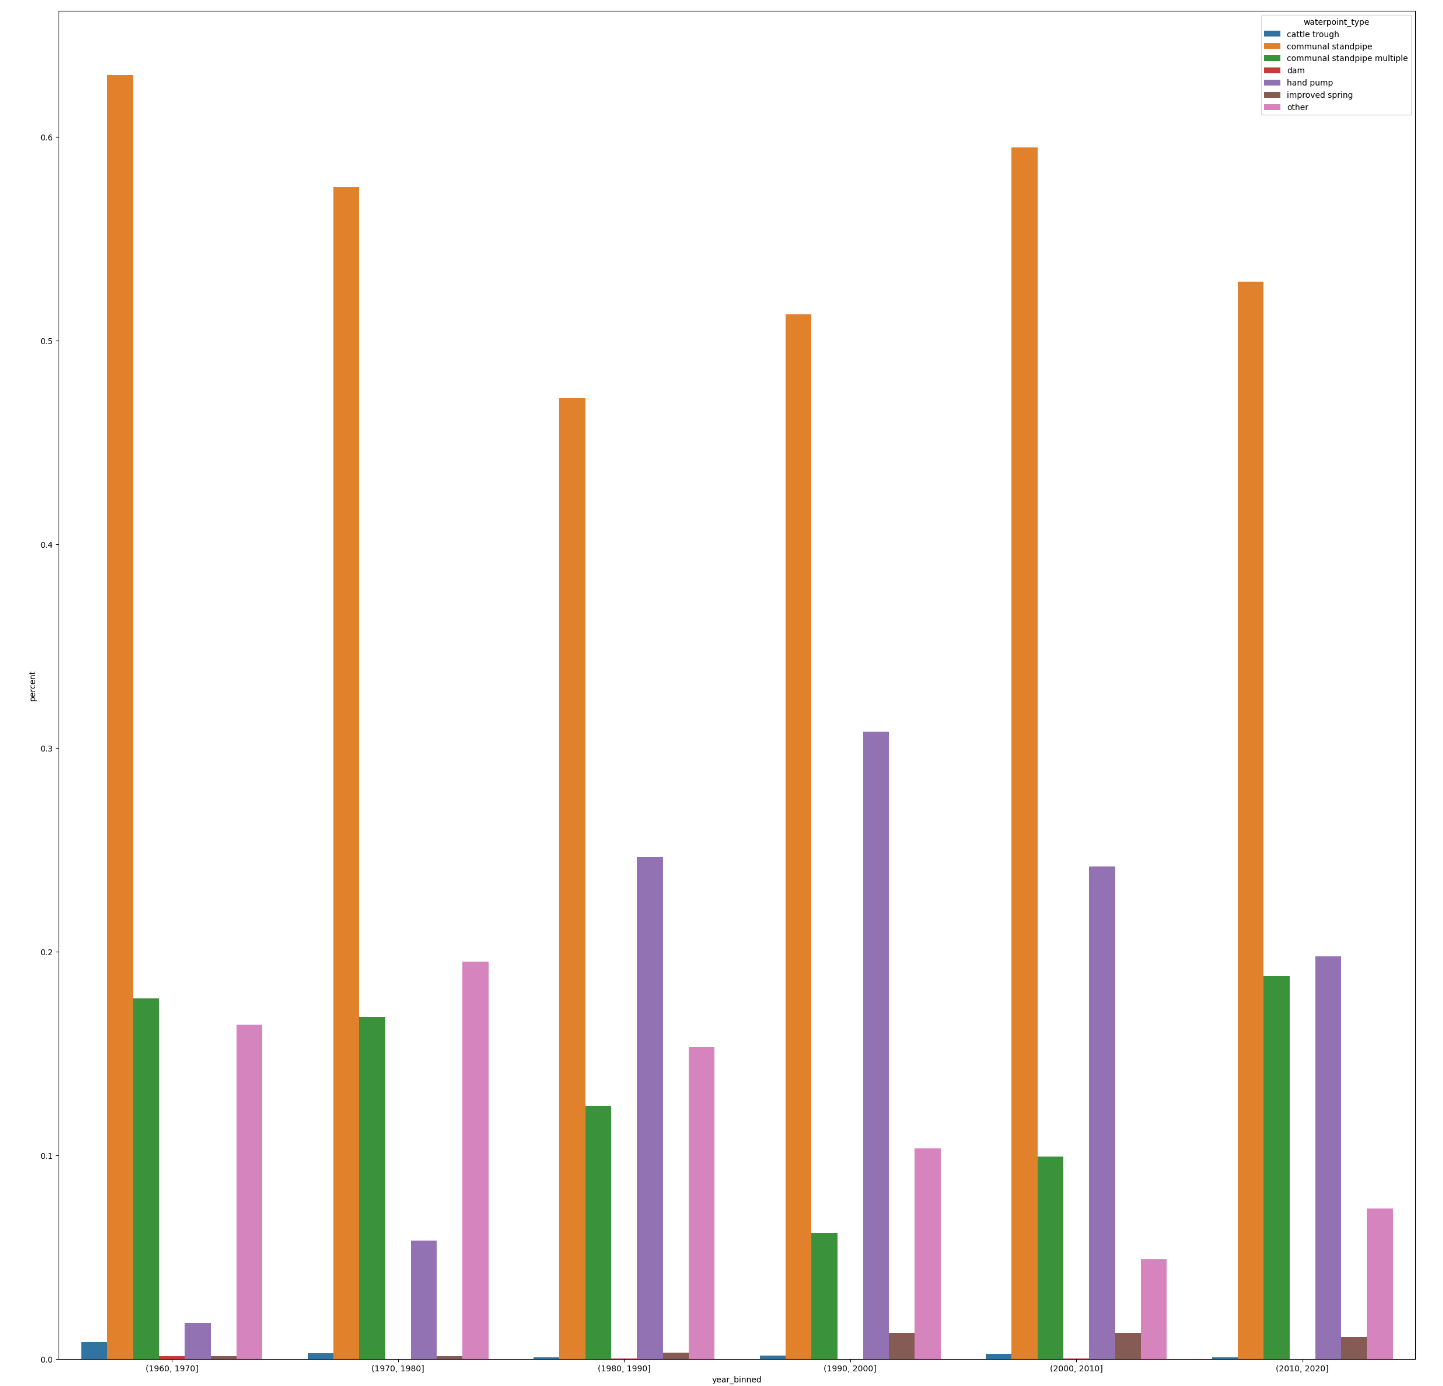
\includegraphics[height=3in]{figures/tom_da_construction_year_1}
      \caption{Waterpoint Type vs Construction Year}
    \end{subfigure}%
    ~
    \begin{subfigure}[t]{0.5\textwidth}
      \centering
      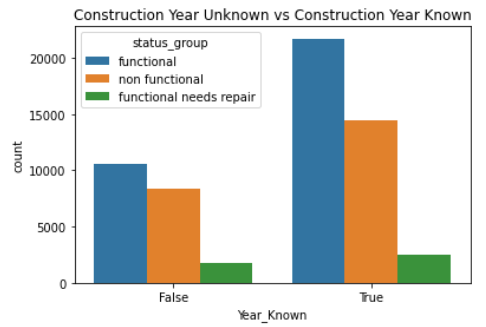
\includegraphics[height=2in]{figures/tom_unknown_cy.png}
      \caption{Construction Year Unknown vs Construction Year Known}
    \end{subfigure}
    ~
    \caption{Construction Year Data Analysis}
    \label{fig:construction_year}
\end{figure*}

\subsubsection{Jason}

Jason analysed the distribution of missing and unique values across all 38 feature columns. One example of this can be seen in Fig \ref{fig:lat_long_distribution}. We can see that each column contains an abnormal amount of a particular value. This will dealt with before training. Furthermore, he had noticed that they were a number of columns that were representing the same thing such as Source \& Source Type. This could be observed in Fig \ref{fig:source}. Other visualisations could be seen in the ipynb notebook submitted with this report.

\begin{figure*}[t]
    \centering
    \begin{subfigure}[t]{0.3\textwidth}
      \centering
      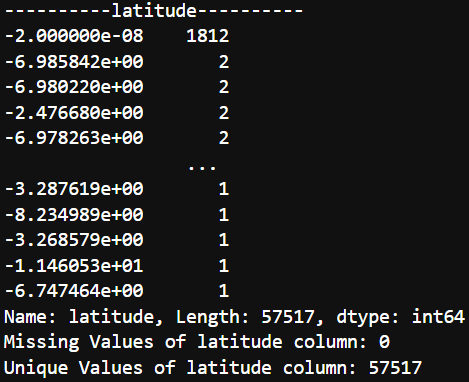
\includegraphics[height=1.5in]{figures/jason_latitude.png}
      \caption{Longitude Distribution}
    \end{subfigure}%
    ~
    \begin{subfigure}[t]{0.3\textwidth}
      \centering
      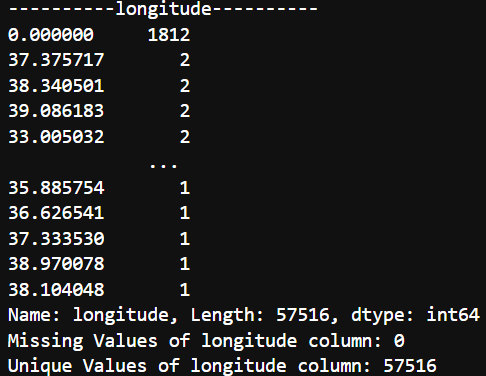
\includegraphics[height=1.5in]{figures/jason_longitude.png}
      \caption{Latitude Distribution}
    \end{subfigure}
    ~
    \caption{Latitude \& Longitude Distribution}
    \label{fig:lat_long_distribution}
\end{figure*}

\begin{figure*}[t]
    \centering
    \begin{subfigure}[t]{0.5\textwidth}
      \centering
      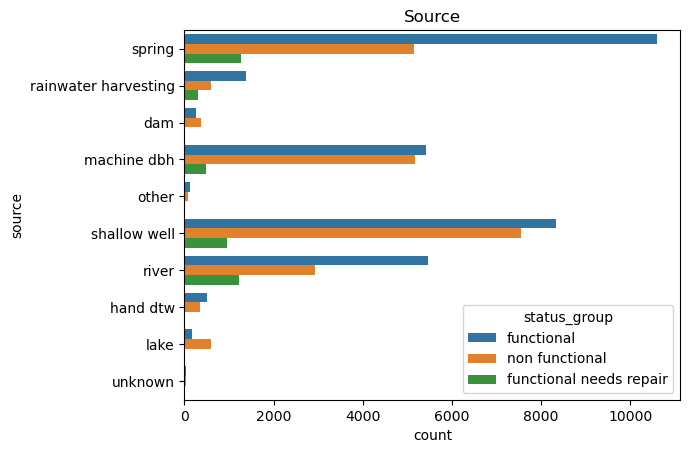
\includegraphics[height=2.25in]{figures/jason_source.png}
      \caption{Source Column Distribution}
    \end{subfigure}%
    ~
    \begin{subfigure}[t]{0.5\textwidth}
      \centering
      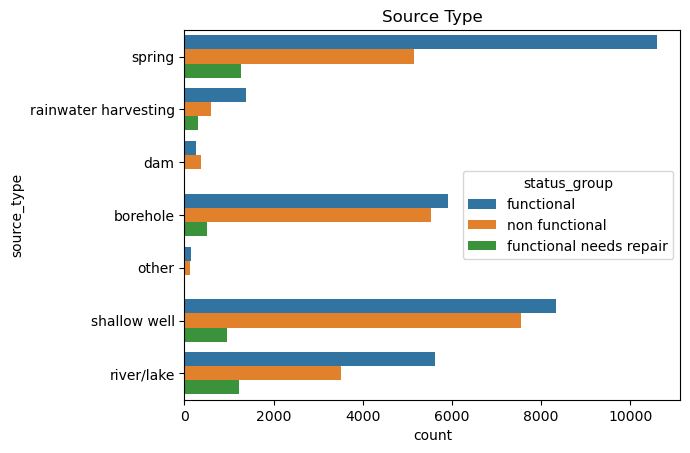
\includegraphics[height=2.25in]{figures/jason_sourcetype.png}
      \caption{Source Type Distribution}
    \end{subfigure}
    ~
    \caption{Well Source Data Analysis}
    \label{fig:source}
\end{figure*}

\subsection{Data Preprocessing}

\subsubsection{Thomas}

Firstly, The results of the latitude and longitude imputation can be seen in Fig. \ref{fig:lat_long_imputation}.

\begin{figure*}[t!]
  \centering
  \begin{subfigure}[t]{0.3\textwidth}
      \centering
      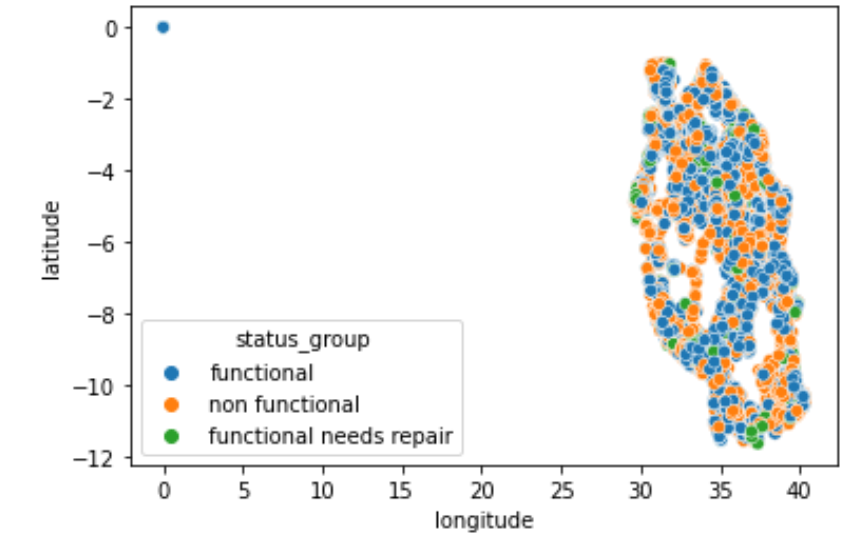
\includegraphics[height=1.45in]{figures/tom_impute_lat_1}
      \caption{Pre-Imputation Latitude \& Longitude}
  \end{subfigure}%
  ~
  \begin{subfigure}[t]{0.3\textwidth}
      \centering
      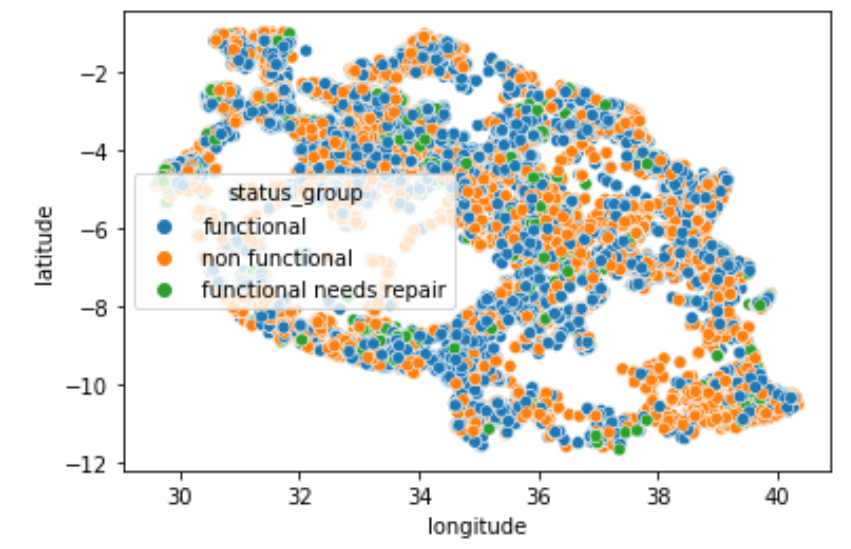
\includegraphics[height=1.5in]{figures/tom_impute_lat_2}
      \caption{Post-Imputation Latitude \& Longitude}
  \end{subfigure}
  ~
  \begin{subfigure}[t]{0.3\textwidth}
      \centering
      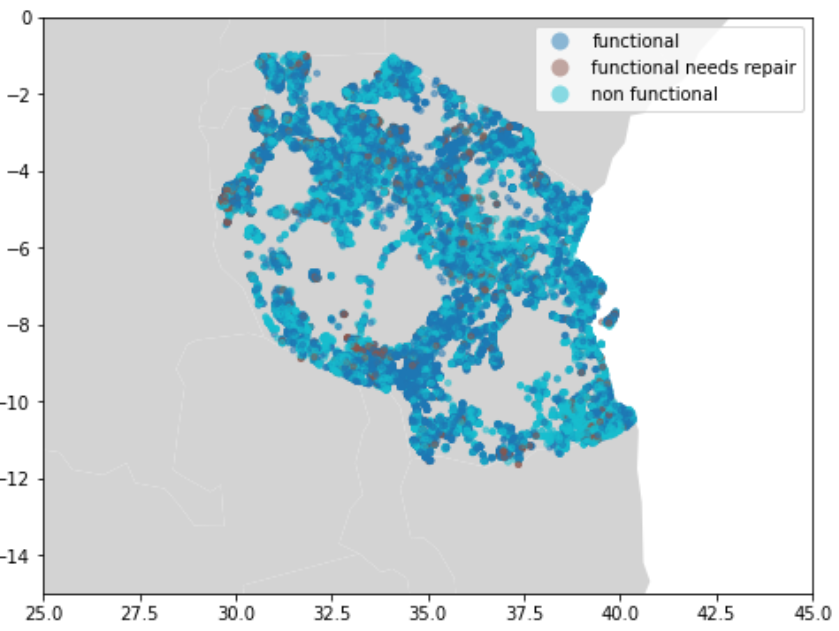
\includegraphics[height=1.5in]{figures/tom_impute_lat_3}
      \caption{Imputated Latitude \& Longitude Overlayed onto a map of Tanzania}
  \end{subfigure}
  ~
  \caption{Latitude \& Longitude Imputation}
  \label{fig:lat_long_imputation}
\end{figure*}

The installer \& funder columns were categorized manually using Thomas' own knowledge and online research. The result was 8 categories, the counts for these are presented in Table \ref{tab:funder_installer_categories}. These versions of the features showed some benefit to the model when testing feature subsets in WandB

\begin{table}[h]
  \centering
  \caption{Funder \& Installer Categories}
  \label{tab:funder_installer_categories}
  \begin{tabular}{|c|c|c|}
    \hline
    Column & Category & Count \\
    \hline
    \multirow{8}{*}{Funder} & Government & 20199 \\
    & Charity & 11066 \\
    & Unknown & 8216 \\
    & Foreign Aid & 8131 \\
    & Religious & 4087 \\
    & Private & 3889 \\
    & Local Government & 3774 \\
    & School & 38 \\
    \hline
    \multirow{8}{*}{Installer} & Local Government & 22515 \\
    & Government & 10327 \\
    & Unknown & 8800 \\
    & Charity & 7487 \\
    & Private & 3853 \\
    & Foreign Aid & 3346 \\
    & Religious & 3046 \\
    & School & 26 \\
    \hline
  \end{tabular}
\end{table}

Thomas used the SMOTE-ENN algorithm to oversample the minority class. The results of this can be seen in Fig. \ref{fig:smote}. On the x-axis, O is 'Functional', '1' is 'Functional - Needs Repair' and 2 is 'Non-Functional'. 

\begin{figure*}[t!]
  \centering
  \begin{subfigure}[t]{0.5\textwidth}
      \centering
      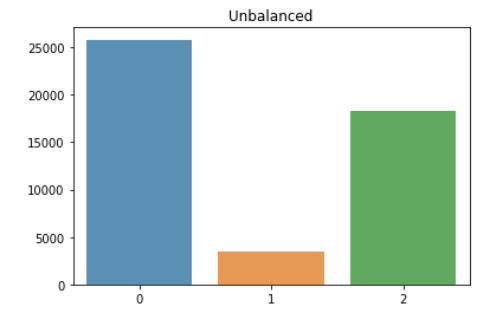
\includegraphics[height=2.25in]{figures/tom_smote_1}
      \caption{Pre-Oversampling Class Distribution}
  \end{subfigure}%
  ~
  \begin{subfigure}[t]{0.5\textwidth}
      \centering
      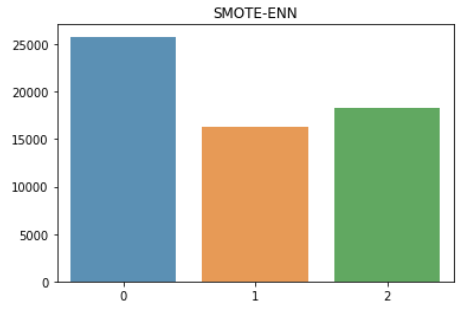
\includegraphics[height=2.25in]{figures/tom_smote_2}
      \caption{Post-Oversampling Class Distribution}
  \end{subfigure}
  ~
  \caption{SMOTE-ENN Oversampling}
  \label{fig:smote}
\end{figure*}

\subsubsection{Jason}

As mentioned in section \ref{ref:method}, Jason performed some pre-processing on the Longitude, Latitude, Public Meeting, Permit, Funder \& Installer columns. The result of funder \& installer columns reclassification could be seen in Table \ref{tab:funder_installer_recategorise}. The graphical representation of the aforementioned pre-processing steps excluding the funder \& installer pre-processing are represented in Fig .\ref{fig:jason_preprocessing}

\begin{figure*}[t!]
  \centering
  \begin{subfigure}[t]{0.225\textwidth}
      \centering
      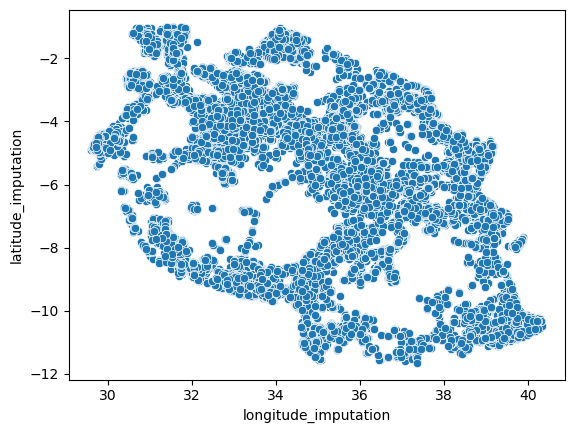
\includegraphics[height=1.35in]{figures/jason_imputation.png}
      \caption{Latitude \& Longitude Mean Imputation}
  \end{subfigure}%
  ~
  \begin{subfigure}[t]{0.225\textwidth}
      \centering
      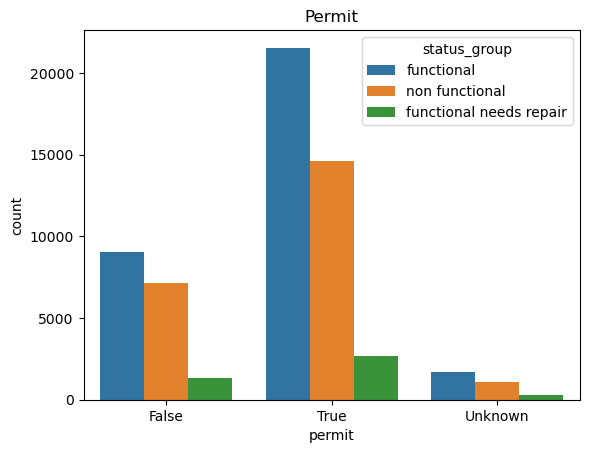
\includegraphics[height=1.35in]{figures/jason_permit.png}
      \caption{Permit Column After Handling Missing Values}
  \end{subfigure}
  ~
  \begin{subfigure}[t]{0.225\textwidth}
      \centering
      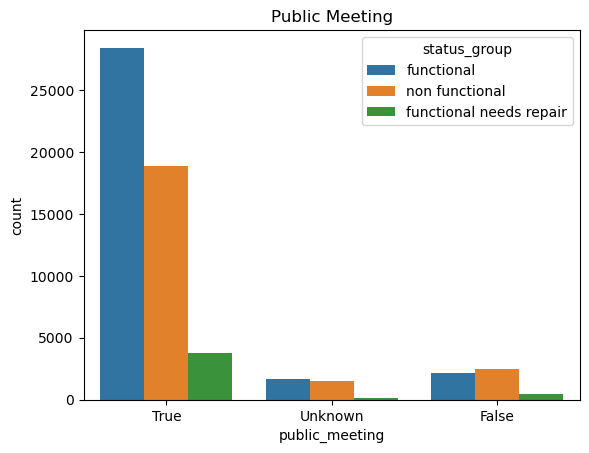
\includegraphics[height=1.35in]{figures/jason_public.png}
      \caption{Public Meeting Column After Handling Missing Values}
  \end{subfigure}
  ~
   \begin{subfigure}[t]{0.225\textwidth}
      \centering
      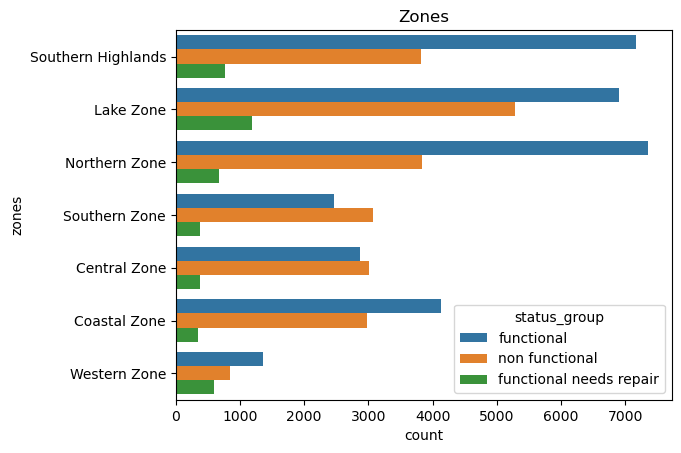
\includegraphics[height=1.35in]{figures/jason_zones.png}
      \caption{Region Column Distribution After Recategorisation}
  \end{subfigure}
  ~
  \caption{Results of Data Pre-processing}
  \label{fig:jason_preprocessing}
\end{figure*}

\begin{table}[]
  \centering
  \caption{Funder \& Installer Recategorise Values}
  \label{tab:funder_installer_recategorise}
  \begin{tabular}{|c|c|c|}
    \hline
    Column & Category & Count \\
    \hline
    \multirow{11}{*}{Funder} & Other & 37405 \\
    & Gov & 9084 \\
    & Danida & 3114 \\
    & Hesawa & 2203 \\
    & ELCT & 1540 \\
    & RWSSP & 1381 \\
    & World Bank & 1349 \\
    & World Vision & 1246 \\
    & Unicef & 1058 \\
    & District Council & 1020\\
    \hline
    \multirow{9}{*}{Installer} & Other & 31828 \\
    & DWE & 17402 \\
    & Gov & 3610 \\
    & Community & 1745 \\
    & Hesawa & 1395 \\
    & RWE & 1206 \\
    & ELCT & 1163 \\
    & Danida & 1051 \\
    \hline
  \end{tabular}
\end{table}

\subsection{Classification} \label{ref:classification_results}

\subsubsection{Thomas}

Post hyper-parameter tuning,accuracy, precision ('macro'), recall ('macro') and f1-score were calculated for each of the models. The models were evaluated on the imbalanced and SMOTE-ENN balanced dataset. The results can be seen in Table \ref{tab:classification_results}

\begin{table*}[t]
  \centering
  \caption{Classification Results}
  \label{tab:classification_results}
  \begin{tabular}{|c|c|c|c|c|c|c|}
    \hline
    \textbf{Scoring} & \textbf{Dataset} & \textbf{Model} & \textbf{Accuracy} & \textbf{Precision} & \textbf{Recall} & \textbf{F1-Score} \\
    \hline
    \multirow{2}{*}{Recall Macro} & \multirow{4}{*}{Balanced} & XGBoost & 0.802 & 0.701 & 0.668 & 0.683 \\
    & & CatBoost & 0.783 & 0.669 & 0.660 & 0.664 \\
    & & HistGradientBoosting & 0.796 & 0.693 & 0.665 & 0.677 \\
    & & BaggingClassifier & 0.803 & 0.703 & \textbf{0.676} & \textbf{0.687} \\
    \cline{2-7}
    & \multirow{4}{*}{Imbalanced} & XGBoost & 0.804 & 0.720 & 0.662 & 0.683 \\
    & & CatBoost & 0.791 & 0.697 & 0.652 & 0.668 \\
    & & HistGradientBoosting & 0.806 & 0.730 & 0.658 & 0.681 \\
    & & BaggingClassifier & 0.803 & 0.722 & 0.660 & 0.681 \\
    \hline
    \multirow{2}{*}{Accuracy} & \multirow{4}{*}{Balanced} & XGBoost & 0.800 & 0.700 & 0.662 &  0.677 \\
    & & CatBoost & 0.787 & 0.678 & 0.665 & 0.670 \\
    & & HistGradientBoosting & 0.797 & 0.699 & 0.666 & 0.680 \\
    & & BaggingClassifier & 0.801 & 0.701 & 0.671 & 0.684 \\
    \cline{2-7}
    & \multirow{4}{*}{Imbalanced} & XGBoost & 0.804 & \textbf{0.748} & 0.648 & 0.676 \\
    & & CatBoost & 0.797 & 0.753 & 0.635 & 0.665\\
    & & HistGradientBoosting & 0.806 & 0.733 & 0.662 & 0.686 \\
    & & BaggingClassifier & \textbf{0.811} & 0.741 & 0.656 & 0.681 \\
    \hline
  \end{tabular}
\end{table*}

The results show the BaggingClassifiers performs the best, although the difference is minimal. The balanced dataset provides a slight increase in F1-Score, which accuracy is higher with the imbalanced dataset. This makes sense, as incorrectly classifying the minority class has a small impact on accuracy but a large impact on F1-Score.

Thomas produced the two confusion matrices using an XGBoost, see Fig. \ref{fig:confusion_matrices}. They show the output of training on both the balanced and imbalanced datasets. Balancing the dataset results in less False Positives on the minority class. If the goal of your model was to do specifically this, perhaps using the balanced dataset would be the best idea. This was not the case for us, so we continued with using the imbalanced dataset.

\begin{figure*}
  \centering
  \begin{subfigure}[t]{0.5\textwidth}
      \centering
      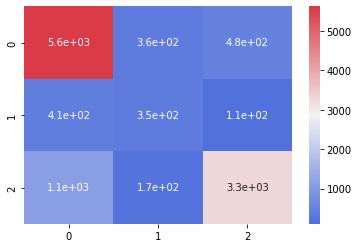
\includegraphics[height=2.25in]{figures/cm_balanced}
      \caption{Balanced Dataset}
  \end{subfigure}%
  ~
  \begin{subfigure}[t]{0.5\textwidth}
      \centering
      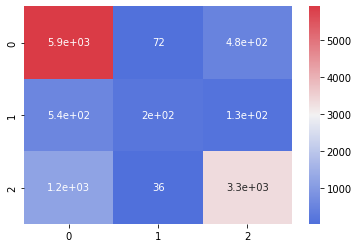
\includegraphics[height=2.25in]{figures/cm_imbalanced}
      \caption{Imbalanced Dataset}
  \end{subfigure}
  ~
  \caption{Balanced vs Imbalanced Confusion Matrices (XGBoost)}
  \label{fig:confusion_matrices}
\end{figure*}

Since the difference between different models and datasets is neglible, Thomas decided to combine all the models to create a VotingClassifier to possibly squeeze out some extra performance. These results can be seen in Table \ref{tab:voting_classification_results}

\begin{table}[H]
  \centering
  \caption{Voting Classifier Results}
  \label{tab:voting_classification_results}
  \begin{tabular}{|c|c|c|c|}
    \hline
    Accuracy & Precision & Recall & F1-Score \\
    \hline
    0.810 & 0.759 & 0.650 & 0.679 \\
    \hline
  \end{tabular}
\end{table}

Using both the results from model based feature selection, and feature selection after looking at the results from Weights \& Biases, Thomas decided to use the following features in his final model: \textbf{'age'}, \textbf{'latitude\_imputation'}, \textbf{'longitude\_imputation'}, \textbf{'construction\_decade'}, \textbf{'quality\_group'}, \textbf{'basin'}, \textbf{'extraction\_type'}, \textbf{'cat\_installer'}, \textbf{'population'}, \textbf{'gps\_height\_zscorenormalise'}, \textbf{'cat\_funder'}, \textbf{'quantity'}, \textbf{'consistent\_water'}, \textbf{'source\_class'}, \textbf{'zones'}, \textbf{'waterpoint\_type'}, \textbf{'season'}, \textbf{'extraction\_type\_class'}, \textbf{'payment'} (Please consult the ipynb for more details on what information these features contain).

To relate this back to our research questions, we can say that these features are the most important when looking at whether wells are functional or not.We can also say we can classify whether a well is function or not with 81\% accuracy.

\subsubsection{Jason}

Based on the results that were obtained from the random forest feature importance and Chi-Squared Test, Jason had decided to use the following features for his model: \textbf{'longitude\_imputation'}, \textbf{'latitude\_imputation'}, \textbf{'quantity'}, \textbf{'extraction\_type\_class'}, \textbf{'gps\_height'}, \textbf{'age'}, \textbf{'waterpoint\_type\_group'}, \textbf{'population\_original'}, \textbf{'payment\_type'}, \textbf{'source\_type'}, \textbf{'funder\_groups'}, \textbf{'basin'}, \textbf{'installer\_grouped'}, \textbf{'management'}, \textbf{'water\_quality'}, \textbf{'public\_meeting'}.

To evaluate the three models that Jason had trained, he decided to use K-fold CV where k=5 and confusion matrices. Important metrics such as precision,recall \& f1-score and K-fold cross validation accuracy score were also calculated. Precision,recall \& f1-score were calculated using macro average. The results of this evaluation can be seen in Table \ref{tab:jason_model}.

\begin{table}[H]
  \centering
  \caption{Trained Model Classification Results}
  \label{tab:jason_model}
  \begin{tabular}{|c|c|c|c|c|}
    \hline
    \textbf{Model} & \textbf{Cross-val Accuracy} & \textbf{Precision} & \textbf{Recall} &\textbf{F1-Score} \\ \hline
    Random Forrest	& 0.795 & 0.72 & 0.64 & 0.67\\
    \hline
    XGBoost &\textbf{0.800} & 0.69 & \textbf{0.67} & \textbf{0.68} \\
    \hline
    CatBoost & 0.787 & \textbf{0.73} & 0.60 & 0.63 \\
    \hline
  \end{tabular}
\end{table}

Receiver Operating Characteristic Curves (ROC) for each model can be seen in Fig \ref{fig:roc_curve}.

\begin{figure*}[t!]
  \centering
  \begin{subfigure}[t]{0.3\textwidth}
      \centering
      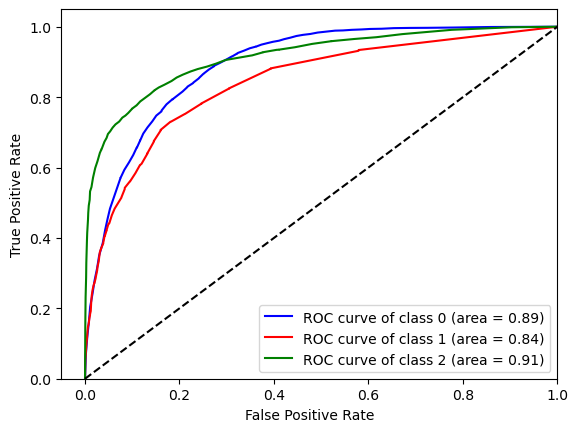
\includegraphics[height=1.65in]{figures/jason_rf.png}
      \caption{Random Forrest ROC Curve}
  \end{subfigure}%
  ~
  \begin{subfigure}[t]{0.3\textwidth}
      \centering
      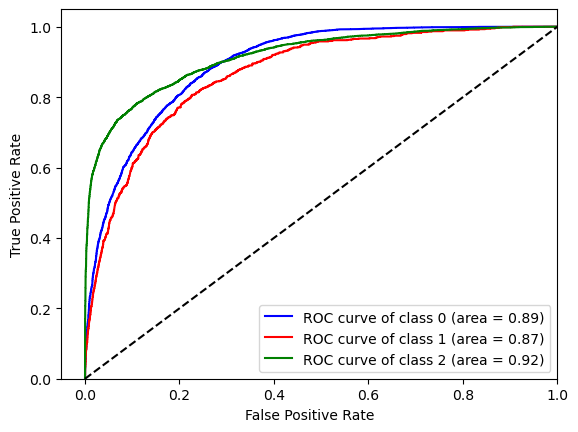
\includegraphics[height=1.65in]{figures/jason_xg.png}
      \caption{XGBoost ROC Curve}
  \end{subfigure}
  ~
  \begin{subfigure}[t]{0.3\textwidth}
      \centering
      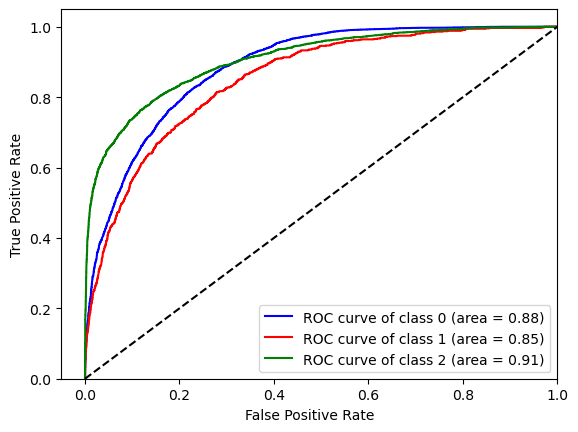
\includegraphics[height=1.65in]{figures/jason_cat.png}
      \caption{CatBoost ROC Curve}
  \end{subfigure}
  ~
  \caption{Models' ROC Curve}
  \label{fig:roc_curve}
\end{figure*}

Out of the 3 models that I had trained throughout this study, I found out that XGBoost performed the best achieving an accuracy of 80\% over Random Forrest (79.5\%) and CatBoost (78.7\%)

\section{Discussion}

In this section, we discuss the results of our analysis. We compare each of our separate approaches to each other, as well as comparing them to the performance of models in the literature.

\subsection{Pre-Processing}

We used many different approaches to pre-processing on this project. One such instance is in terms of scaling. Tom applied a MinMaxScaler only on one feature 'gps\_height'. However, Jason applied Z-Score Normalisation on every feature. Despite the presence of categorical data, Jason's method still produced high quality results. Our models performed equally, achieving an accuracy of 81\% and 80\%. This indicates that both normalisation methods could be considered acceptable in this study.

Another aspect that was different was the handling of the funder \& installer columns. Jason decided to first fix the spelling mistakes before proceeding to classifying those unique values with value counts above 1000 as its own individual class while those below that threshold would be classified under the "Other" class. Tom decided to individually classify them in categories based on research. By doing this, Tom lost valuable information but not using the specific funders or installers. Jason's approach lost less information as only values with small counts were removed from the dataset and classified as "Other". Jason's technique proved slightly better.

One of the differences that could be observed in the Pre-processing stage of this study is the way we implemented mean imputation for the missing values in longitude \& latitude columns. Jason decided to utilise a simpler approach where the value was imputed based on a region's average value. However, Tom decided to impute them based on the order of 'ward', 'lga' and 'region'. Tom's method in theory should represent the data distribution better as it takes more specific features such as 'ward' \& 'lga' which are smaller than 'region'. The simpler approach that Jason took could skew the data towards the mean of a region which could result in some data being lost. But during model evaluation it was noted that the simpler approach resulted in better performance.



\subsection{Modelling}

The choice of hyper-parameter tuning methods between the two of us showcased the different ideologies that we had. Jason opted for a smaller but in depth search space with GridSearch while Tom opted for a broad but shallower search space with RandomSearch. RandomSearch enabled a wider exploration of hyperparameter ranges across various models, making it faster. On the other hand, GridSearch focused on specific potential hyperparameters, providing a more in-depth search. This is reflected in our results, as Jason's XGBoost out-performed Tom's XGBoost, yet the breadth of search allowed Tom to find the BaggingClassifier which performed well. Tom's VotingClassifier slightly edged Jason's XGBoost in terms of accuracy (81\% vs 80\%).


\subsubsection{Jason}

Tom started by modelling baseline models involving different algorithms without feature selection to gauge the performance of each model on this dataset. This was in contrast what I did as I already had an idea on what models to develop. Tom's method actually gave a better insight on the models that could potentially be suited for this dataset. This allowed him to narrow down the models that he should try to developed. I noticed that rushing towards the development of a model directly without any testing like what I did was unwise as it could lead to valuable time being wasted on models that do not perform well on this dataset.

When we consider the models that both of us had trained, I find Tom's implementation of a VotingClassifer rather interesting. Instead of developing a model that utilised only one algorithm, he decided to combine his developed XGBoost, CatBoost, HistGradientBoosting and BaggingClassifier into a VotingClassifier. All three models were used to make predictions on unseen data and the algorithm that had the best performance would be selected to make the classification. A VotingClassifier in this scenario could be seen as more robust in comparison with models that only  utilise one algorithm. The results from this study further echo the above sentiment with Tom's VotingClassifier achieving better performance than my XGBoost.

\subsubsection{Tom}

Jason performed more analysis of his models than myself. I think this led to more iterative improvements. In my cases, post hyper-parameter tuning the models were simply evaluated on the test set using Accuracy \& F1-Score. However, Jason used K-Fold CV and ROC Curves to really understand his models, and I think in the long run this resulted in improved performance. He could accurately see where his models required improvement.

Jason also produced a much more thorough statistical analysis, which I would have struggled without. I thank our 'Christmas-Tree' management approach for this insight, as Jason was able to share information with me I would not have be able to find otherwise.


\section{Conclusion}

Overall, we have successfully developed and evaluated 8 different ML models on the Pump It Up dataset. Tom's VotingClassifier performed the best with a classification accuracy of 81\%. Our  models have successfully showcased the feasibility of applying machine learning to aid the Tanzanian Government in classifying the status of wells based on historical data. Through machine learning, the Tanzanian Government would be able to act quicker in identifying and repairing wells that are non functional for the benefit of their people. 

One of the shortcomings of this study is that the dataset provided was incomplete and had invalid values. Important values such as construction year which would typically affect the status of a well was missing in the regions of 20,000s. Although imputation was done to mitigate the effects of invalid data, it is still not a proper representation of the data that the ML would be faced with during deployment.

Unfortunately, one of our supplementary research questions: \textbf{Could we use our results to ensure that the wells are built and repaired so that fewer wells are non functional?} was not answered in this study due to the lack of relevant data in the Pump It Up dataset. Moving forward, we seek to obtain additional data from Taarifa and Tanzanian Ministry of Water to be able to calculate the lifetime and decay rate of wells as mentioned by Pham et al \cite{Pham_2018}. Both of these metrics would allow us to have a better understanding of the lifetime of a well and how long it takes for a well to be non functional. Furthermore, we would like to explore the possibility of applying more state of the art ML models i.e. Transformers on the Pump It Up dataset as only traditional ML models were considered in this study. 

\section{Contributions}

We each contributed equally. For the programming, please view the comments at the top of each cell of the submitted notebook to see the author. In the report, Thomas wrote the Literature Review in the report, and Jason did the conclusion. We worked on the remaining sections together.

\bibliographystyle{IEEEtran}
\bibliography{refs}

\end{document}